\hypertarget{gemoda-r_8c}{
\section{gemoda-r.c File Reference}
\label{gemoda-r_8c}\index{gemoda-r.c@{gemoda-r.c}}
}
{\tt \#include \char`\"{}bit\-Set.h\char`\"{}}\par
{\tt \#include \char`\"{}convll.h\char`\"{}}\par
{\tt \#include \char`\"{}Fasta\-Seq\-IO/fasta\-Seq\-IO.h\char`\"{}}\par
{\tt \#include $<$unistd.h$>$}\par
{\tt \#include $<$stdlib.h$>$}\par
{\tt \#include $<$errno.h$>$}\par
{\tt \#include $<$string.h$>$}\par
{\tt \#include \char`\"{}real\-Io.h\char`\"{}}\par
{\tt \#include \char`\"{}real\-Compare.h\char`\"{}}\par


Include dependency graph for gemoda-r.c:\begin{figure}[H]
\begin{center}
\leavevmode
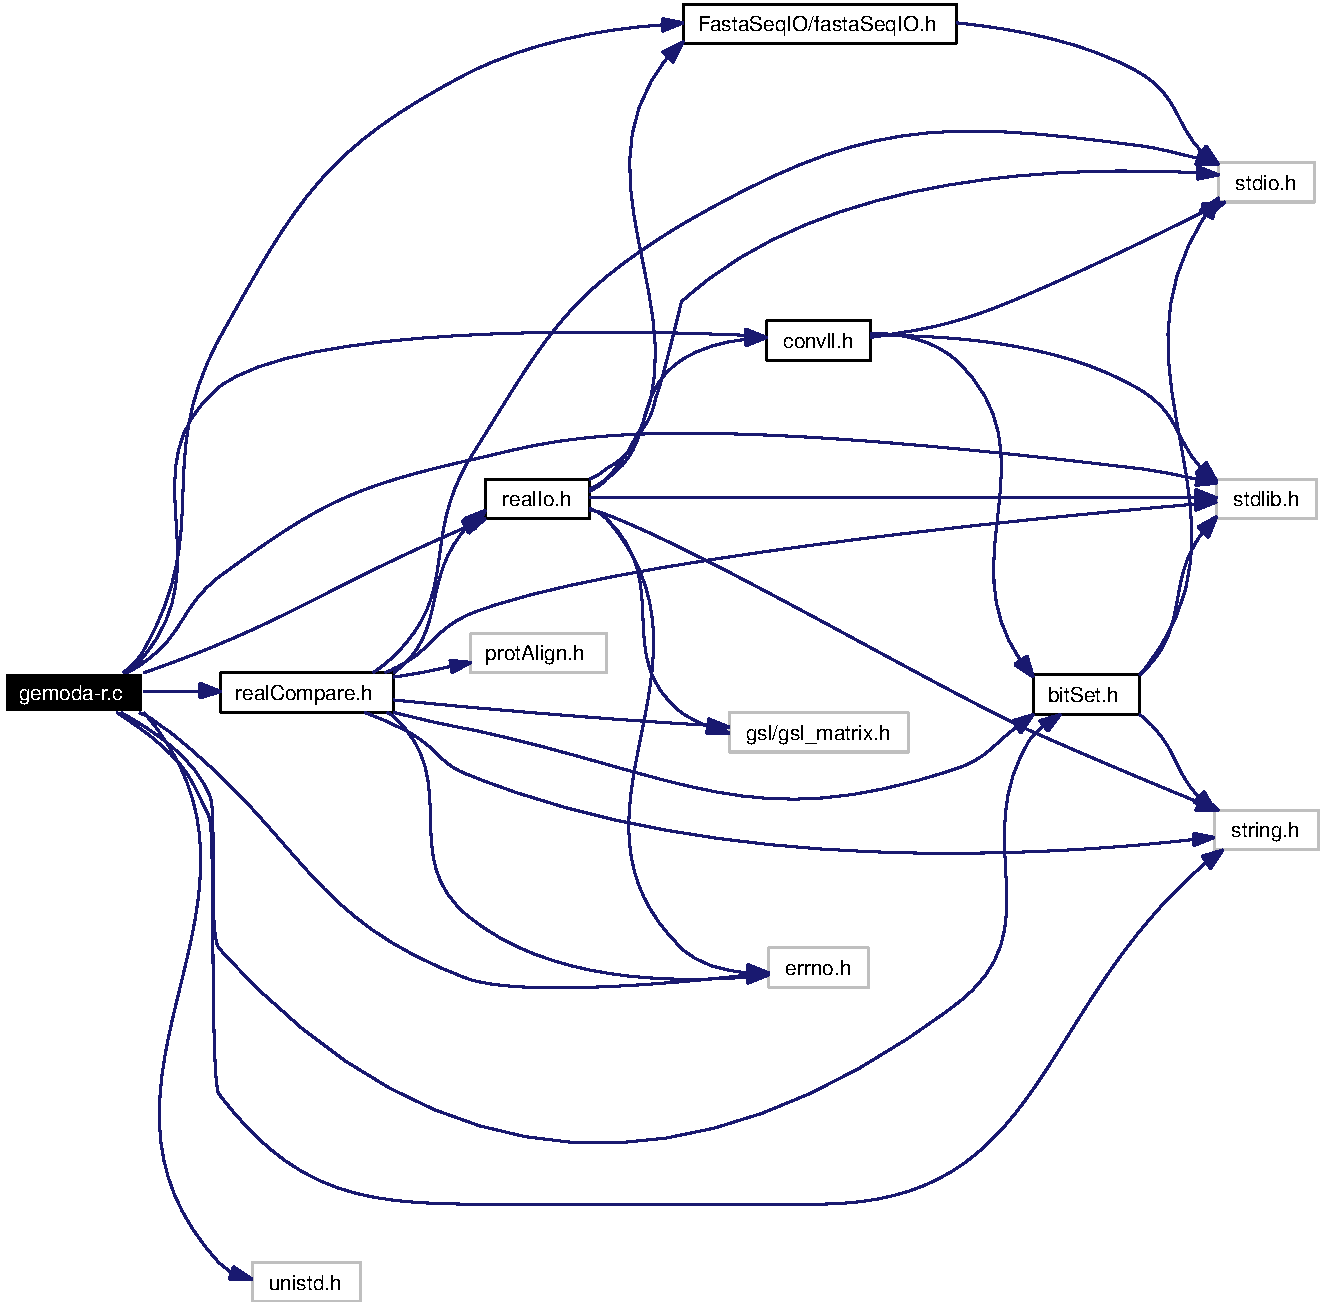
\includegraphics[width=334pt]{gemoda-r_8c__incl}
\end{center}
\end{figure}
\subsection*{Functions}
\begin{CompactItemize}
\item 
void \hyperlink{gemoda-r_8c_a0}{usage} (char $\ast$$\ast$argv)
\item 
\hyperlink{structcnode}{cll\_\-t} $\ast$ \hyperlink{gemoda-r_8c_a1}{convolve} (\hyperlink{structbitGraph__t}{bit\-Graph\_\-t} $\ast$bg, int support, int R, int $\ast$index\-To\-Seq, int p, int cluster\-Method, int $\ast$$\ast$offset\-To\-Index, int number\-Of\-Sequences, int no\-Convolve, FILE $\ast$OUTPUT\_\-FILE)
\item 
\hyperlink{structbitGraph__t}{bit\-Graph\_\-t} $\ast$ \hyperlink{gemoda-r_8c_a2}{prune\-Bit\-Graph} (\hyperlink{structbitGraph__t}{bit\-Graph\_\-t} $\ast$bg, int $\ast$index\-To\-Seq, int $\ast$$\ast$offset\-To\-Index, int num\-Of\-Seqs, int p)
\item 
int \hyperlink{gemoda-r_8c_a3}{count\-Extra\-Params} (char $\ast$s)
\item 
double $\ast$ \hyperlink{gemoda-r_8c_a4}{parse\-Extra\-Params} (char $\ast$s, int num\-Params)
\item 
int \hyperlink{gemoda-r_8c_a5}{main} (int argc, char $\ast$$\ast$argv)
\end{CompactItemize}


\subsection*{Detailed Description}
This file contains the main routine for the real valued version of Gemoda. There are also some accessory functions for printing information on how to use Gemoda and run it from the commandline.

Definition in file \hyperlink{gemoda-r_8c-source}{gemoda-r.c}.

\subsection*{Function Documentation}
\hypertarget{gemoda-r_8c_a1}{
\index{gemoda-r.c@{gemoda-r.c}!convolve@{convolve}}
\index{convolve@{convolve}!gemoda-r.c@{gemoda-r.c}}
\subsubsection[convolve]{\setlength{\rightskip}{0pt plus 5cm}\hyperlink{structcnode}{cll\_\-t}$\ast$ convolve (\hyperlink{structbitGraph__t}{bit\-Graph\_\-t} $\ast$ {\em bg}, int {\em support}, int {\em R}, int $\ast$ {\em index\-To\-Seq}, int {\em p}, int {\em cluster\-Method}, int $\ast$$\ast$ {\em offset\-To\-Index}, int {\em number\-Of\-Sequences}, int {\em no\-Convolve}, FILE $\ast$ {\em OUTPUT\_\-FILE})}}
\label{gemoda-r_8c_a1}


Our outer convolution function. This function will call preliminary functions, cluster the data, and then call the main convolution function. This is the interface between the main gemoda-$<$x$>$ code and the generic code that gets all of the work done. Input: the bit\-Graph to be clustered and convolved, the minimum support necessary for a motif to be returned, a flag indicating whether recursive filtering should be used, a pointer to the data structure that dereferences offset indices to sequence numbers, the number of unique source sequences that a motif must be present in, and a number indicating the clustering method that is to be used. Output: the final motif linked list with all motifs that are to be given as output to the user.

Definition at line 625 of file new\-Conv.c.

Referenced by main().

\scriptsize\begin{verbatim}629 {
630   bitSet_t * cand = NULL;
631   bitSet_t * mask = NULL;
632   bitSet_t * Q = NULL;
633   int size = bg->size;
634   cll_t * elemPats = NULL;
635   cll_t * allCliques = NULL;
636   cll_t * curr = NULL;
637   
638     // contains indices (rows) containing the threshold value.
639     cand = newBitSet (size);
640   mask = newBitSet (size);
641   Q = newBitSet (size);
642   fillSet (cand);
643   fillSet (mask);
644   
645     // Note that we prune based on p before setting the diagonal false.
646     if (p > 1)
647     {
648       bg =
649     pruneBitGraph (bg, indexToSeq, offsetToIndex, numberOfSequences, p);
650     }
651   
652     // Now we set the main diagonal false for clustering and filtering.
653     bitGraphSetFalseDiagonal (bg);
654   filterGraph (bg, support, R);
655   fprintf (OUTPUT_FILE, "Graph filtered!  Now clustering...\n");
656   fflush (NULL);
657   if (clusterMethod == 0)
658     {
659       findCliques (Q, cand, mask, bg, support, 0, &elemPats, indexToSeq, p);
660     }
661   else
662     {
663       singleLinkage (Q, cand, mask, bg, support, 0, &elemPats, indexToSeq,
664               p);
665     }
666   fprintf (OUTPUT_FILE,
667         "Clusters found!  Now filtering clusters (if option set)...\n");
668   fflush (NULL);
669   if (p > 1)
670     {
671       elemPats = pruneCll (elemPats, indexToSeq, p);
672     }
673   deleteBitSet (cand);
674   deleteBitSet (mask);
675   deleteBitSet (Q);
676   
677     // Now let's convolve what we made.
678     if (noConvolve == 0)
679     {
680       fprintf (OUTPUT_FILE, "Now convolving...\n");
681       fflush (NULL);
682       allCliques = completeConv (&elemPats, support, size, 0, indexToSeq, p);
683     }
684   
685   else
686     {
687       curr = elemPats;
688       while (curr != NULL)
689     {
690       yankCll (&elemPats, NULL, &curr, &allCliques, 0);
691     }
692     }
693   return allCliques;
694 }
\end{verbatim}
\normalsize 


\hypertarget{gemoda-r_8c_a3}{
\index{gemoda-r.c@{gemoda-r.c}!countExtraParams@{countExtraParams}}
\index{countExtraParams@{countExtraParams}!gemoda-r.c@{gemoda-r.c}}
\subsubsection[countExtraParams]{\setlength{\rightskip}{0pt plus 5cm}int count\-Extra\-Params (char $\ast$ {\em s})}}
\label{gemoda-r_8c_a3}




Definition at line 91 of file gemoda-r.c.

Referenced by main().

\scriptsize\begin{verbatim}92 {
93   int i = 0;
94   int numParams = 1;
95   for (i = 0; i < strlen (s); i++)
96     {
97       if (s[i] == ',')
98     {
99       numParams++;
100     }
101     }
102   return numParams;
103 }
\end{verbatim}
\normalsize 


\hypertarget{gemoda-r_8c_a5}{
\index{gemoda-r.c@{gemoda-r.c}!main@{main}}
\index{main@{main}!gemoda-r.c@{gemoda-r.c}}
\subsubsection[main]{\setlength{\rightskip}{0pt plus 5cm}int main (int {\em argc}, char $\ast$$\ast$ {\em argv})}}
\label{gemoda-r_8c_a5}


This is the main routine of the real value Gemoda code. The code runs similarly to the sequence Gemoda code: there is a comparison phase, followed by a clustering phase, followed by a convolution phase. Only the comparison phase is unique to the real value Gemoda. Of course, since the data are formatted so differently, there are vastly different pieces of code in the front matter. In particular, there is no hashing of words obviously. As well, we use the GNU scientific library to store real value data as matrices that can be easily manipulated.

Definition at line 160 of file gemoda-r.c.

References calc\-Stat\-All\-Cliqs(), convolve(), count\-Extra\-Params(), cum\-DMatrix(), delete\-Bit\-Graph(), free\-D(), free\-Rdh(), get\-Stat\-Mat(), rdh\_\-t::index\-To\-Seq, rdh\_\-t::offset\-To\-Index, output\-Real\-Pats(), output\-Real\-Pats\-WCentroid(), parse\-Extra\-Params(), pop\-All\-Cll(), read\-Real\-Data(), real\-Comparison(), bit\-Graph\_\-t::size, rdh\_\-t::size, sort\-By\-Stats(), and usage().

\scriptsize\begin{verbatim}161 {
162   int inputOption = 0;
163   char *sequenceFile = NULL;
164   FILE *SEQUENCE_FILE = NULL;
165   char *outputFile = NULL;
166   FILE *OUTPUT_FILE = NULL;
167   int L = 0;
168   int status = 0;
169   double g = 0;
170   int sup = 2;
171   int R = 1;
172   int P = 0;
173   int compFunc = 0;
174   double *extraParams = NULL;
175   int numExtraParams = 0;
176   int i = 0, j = 0;
177   /*
178      int j, k, i, l;
179    */
180   int noConvolve = 0;
181   int samp = 1;
182   int supportDim = 0, lengthDim = 0;
183   bitGraph_t *oam = NULL;
184   unsigned int **d = NULL;
185   int oamSize = 0;
186 
187   cll_t *allCliques = NULL;
188   /*
189      cll_t *curCliq = NULL;
190    */
191   /*
192      int curSeq;
193    */
194   /*
195      int curPos;
196    */
197   int clusterMethod = 0;
198   int joelOutput = 0;
199 
200   // gemoda-r new stuff
201   rdh_t *data = NULL;
202 
203   /*
204      Get command-line options 
205    */
206   while ((inputOption = getopt (argc, argv, "p:m:e:i:o:l:g:k:c:njs:")) != EOF)
207     {
208       switch (inputOption)
209     {
210       // Comparison metric
211     case 'm':
212       compFunc = atoi (optarg);
213       break;
214       // Input file
215     case 'i':
216       sequenceFile = optarg;
217       break;
218       // Output file
219     case 'o':
220       outputFile =
221         (char *) malloc ((strlen (optarg) + 1) * sizeof (char));
222       if (outputFile == NULL)
223         {
224           fprintf (stderr, "Error allocating memory for options.\n");
225           exit (EXIT_FAILURE);
226         }
227       else
228         {
229           strcpy (outputFile, optarg);
230         }
231       break;
232       // Minimum motif length
233     case 'l':
234       L = atoi (optarg);
235       break;
236       // Minimum motif similarity score
237     case 'g':
238       g = atof (optarg);
239       status++;
240       break;
241       // Minimum support (number of motif occurrences)
242     case 'k':
243       sup = atoi (optarg);
244       break;
245 
246 /***************************************************************
247  * Recursive initial pruning: an option for clique finding.
248  *   It takes all nodes with less than the minimum
249  *   number of support and removes all of their nodes, and does this 
250  *   recursively so that nodes that are connected to many sparsely connected
251  *   nodes will be removed and not left in the 
252  * This option is deprecated as it is at worst no-gain and at best useful.
253  *   It will be on by default for clique-finding, but can be turned 
254  *   back off with some
255  *   minor tweaking.  For almost all cases in which it does not speed
256  *   up computations, it will have a trivial time to perform.  Thus, if 
257  *   clique-finding is turned on, then R is set to 1 by default.
258         case 'r':
259             R = 1;
260             break;
261 ************************************************************************/
262       // Optional pruning parameter to require at motif occurrences
263       // in at least P distinct input sequences
264 
265     case 'p':
266       P = atoi (optarg);
267       break;
268 
269       // Clustering method.
270     case 'c':
271       clusterMethod = atoi (optarg);
272       break;
273       // Extra parameters for comparison function
274     case 'e':
275       numExtraParams = countExtraParams (optarg);
276       extraParams = parseExtraParams (optarg, numExtraParams);
277       break;
278     case 'n':
279       noConvolve = 1;
280       break;
281     case 'j':
282       joelOutput = 1;
283       break;
284     case 's':
285       samp = atoi (optarg);
286       break;
287       // Catch-all.
288     case '?':
289       fprintf (stderr, "Unknown option `-%c'.\n", optopt);
290       usage (argv);
291       return EXIT_SUCCESS;
292     default:
293       usage (argv);
294       return EXIT_SUCCESS;
295     }
296     }
297   // Require an input file, a nonzero length, and a similarity threshold
298   // to be set.
299   if (sequenceFile == NULL || L == 0 || status < 1)
300     {
301       usage (argv);
302       return EXIT_SUCCESS;
303     }
304   // Open the sequence file
305   if ((SEQUENCE_FILE = fopen (sequenceFile, "r")) == NULL)
306     {
307       fprintf (stderr, "Couldn't open file %s; %s\n", sequenceFile,
308            strerror (errno));
309       exit (EXIT_FAILURE);
310     }
311   // Open the output file
312   if (outputFile != NULL)
313     {
314       if ((OUTPUT_FILE = fopen (outputFile, "w")) == NULL)
315     {
316       fprintf (stderr, "Couldn't open file %s; %s\n", outputFile,
317            strerror (errno));
318       exit (EXIT_FAILURE);
319     }
320     }
321   else
322     {
323       OUTPUT_FILE = stdout;
324     }
325 
326 
327 
328   // Verbosity in output helps to distinguish output files.
329   fprintf (OUTPUT_FILE, "Input file = %s\n", sequenceFile);
330   fprintf (OUTPUT_FILE, "l = %d, k = %d, g = %f\n", L, sup, g);
331   if (P > 1)
332     {
333       fprintf (OUTPUT_FILE, "Minimum # of sequences with motif = %d\n", P);
334     }
335   if (R > 0)
336     {
337       fprintf (OUTPUT_FILE, "Recursive pruning is ON.\n");
338     }
339 
340   data = readRealData (SEQUENCE_FILE);
341   fclose (SEQUENCE_FILE);
342   // printf("size = %d,indexSize = %d\n",data->size,data->indexSize);
343   // printf("size1 = %d,size2 = %d\n",data->seq[0]->size1,data->seq[0]->size2);
344   // for(i = 0; i < 2; i++) {
345   // for(j = 0; j < 3; j++) {
346   // printf("%lf,%lf,%lf\n",gsl_matrix_get(data->seq[i],j,0),
347   // gsl_matrix_get(data->seq[i],j,1),
348   // gsl_matrix_get(data->seq[i],j,2));}}
349   oam = realComparison (data, L, g, compFunc, extraParams);
350   // printf("oam->size = %d\n", oam->size);
351   if ((samp > 0) && (clusterMethod == 0))
352     {
353       // We are currently using one gap per sequence, as done in 
354       // realCompare.c's call to initRdhIndex in realComparison.
355       // Note that this is data->size, NOT oam->size.
356       d =
357     getStatMat (oam, sup, L, &supportDim, &lengthDim, data->size, samp,
358             OUTPUT_FILE);
359     }
360   else
361     {
362       d = NULL;
363       supportDim = 0;
364     }
365 
366   allCliques =
367     convolve (oam, sup, R, data->indexToSeq, P, clusterMethod,
368           data->offsetToIndex, data->size, noConvolve, OUTPUT_FILE);
369 
370   oamSize = oam->size;
371   // Do some early memory cleanup since this is so big.
372   deleteBitGraph (oam);
373 
374   if ((samp > 0) && (clusterMethod == 0))
375     {
376       cumDMatrix (d, allCliques, supportDim, lengthDim, oamSize, data->size);
377       calcStatAllCliqs (d, allCliques, oamSize - data->size);
378       allCliques = sortByStats (allCliques);
379     }
380 
381   if (joelOutput == 0)
382     {
383       outputRealPats (data, allCliques, L, OUTPUT_FILE, d);
384     }
385   else
386     {
387       outputRealPatsWCentroid (data, allCliques, L, OUTPUT_FILE, extraParams,
388                    compFunc);
389     }
390 
391   freeD (d, supportDim);
392   freeRdh (data);
393   allCliques = popAllCll (allCliques);
394   fclose (OUTPUT_FILE);
395 
396   return 0;
397 }
\end{verbatim}
\normalsize 


\hypertarget{gemoda-r_8c_a4}{
\index{gemoda-r.c@{gemoda-r.c}!parseExtraParams@{parseExtraParams}}
\index{parseExtraParams@{parseExtraParams}!gemoda-r.c@{gemoda-r.c}}
\subsubsection[parseExtraParams]{\setlength{\rightskip}{0pt plus 5cm}double$\ast$ parse\-Extra\-Params (char $\ast$ {\em s}, int {\em num\-Params})}}
\label{gemoda-r_8c_a4}


This was borrowed from the old gemoda-p code, there it used to parse filenames, here we are parsing comma-separated lists of doubles that are useful for Spec\-Connect.

Definition at line 110 of file gemoda-r.c.

Referenced by main().

\scriptsize\begin{verbatim}111 {
112   int i = 0, j = 0, k = 0;
113   int startLength = 0;
114   double *extraParams = NULL;
115   char *paramString = NULL;
116 
117   extraParams = (double *) malloc (numParams * sizeof (double));
118   if (extraParams == NULL)
119     {
120       fprintf (stderr, "Can't allocate extra params!\n");
121       exit (0);
122     }
123   j = 0;
124   k = 0;
125   startLength = strlen (s);
126   for (i = 0; i < startLength; i++)
127     {
128       if (s[i] == ',')
129     {
130       // We've found an end.  So point the pointer to
131       // the beginning of the previous string.
132       paramString = &s[k];
133       // Terminate the string where the comma used to be
134       s[i] = '\0';
135       // Update the location for the next string beginning
136       k = i + 1;
137       // Convert to a double and update the param number.
138       extraParams[j] = atof (paramString);
139       j++;
140     }
141     }
142   // Don't forget to do the last one, which isn't comma-terminated.
143   paramString = &s[k];
144   extraParams[j] = atof (paramString);
145   return (extraParams);
146 }
\end{verbatim}
\normalsize 


\hypertarget{gemoda-r_8c_a2}{
\index{gemoda-r.c@{gemoda-r.c}!pruneBitGraph@{pruneBitGraph}}
\index{pruneBitGraph@{pruneBitGraph}!gemoda-r.c@{gemoda-r.c}}
\subsubsection[pruneBitGraph]{\setlength{\rightskip}{0pt plus 5cm}\hyperlink{structbitGraph__t}{bit\-Graph\_\-t}$\ast$ prune\-Bit\-Graph (\hyperlink{structbitGraph__t}{bit\-Graph\_\-t} $\ast$ {\em bg}, int $\ast$ {\em index\-To\-Seq}, int $\ast$$\ast$ {\em offset\-To\-Index}, int {\em num\-Of\-Seqs}, int {\em p})}}
\label{gemoda-r_8c_a2}


Simple function (non-recursive) to prune off the first level of motifs that will not meet the \char`\"{}minimum number of unique sequences\char`\"{} criterion. This could have been implemented as above, but it may have gotten a little expensive with less yield, so only the first run through is done here. Input: a bit graph to be pruned, a pointer to the structure that dereferences offset indices to sequence numbers, a pointer to the structure that dereferences seq/position to offsets, the number of unique sequences in the input set, and the minimum number of unique sequences that must contain the motif. Output: a pruned bit\-Graph.

Definition at line 402 of file new\-Conv.c.

Referenced by convolve().

\scriptsize\begin{verbatim}404 {
405   int i = 0, j = 0, nextBit = 0;
406   int *seqNums = NULL;
407   
408     // Since we don't immediately know which node is in which source 
409     // sequence, we can't just count them up regularly.  Instead, we'll
410     // need to keep track of which sequences they come from and 
411     // increment _something_.  What we chose to do here is just make
412     // an array of integers of length = <p>.  Then, we try to put the
413     // source sequence number of each neighbor (including itself, since
414     // the main diagonal is still true at this time) into the next slot
415     // Since we will monotonically search the bitSet, we can just 
416     // move on to the first bit in the next sequence using the 
417     // offsetToIndex structure so that we know the next sequence number
418     // to be put in is always unique.
419     seqNums = (int *) malloc (p * sizeof (int));
420   if (seqNums == NULL)
421     {
422       fprintf (stderr, "Memory error - pruneBitGraph\n%s\n",
423         strerror (errno));
424       fflush (stderr);
425       exit (0);
426     }
427   
428     // So, for each row in the bitgraph...
429     for (i = 0; i < bg->size; i++)
430     {
431       
432     // Make sure the whole array is -1 sentinels.
433     for (j = 0; j < p; j++)
434     {
435       seqNums[j] = -1;
436     }
437       j = 0;
438       
439     // Find the first neighbor of this bit.
440     nextBit = nextBitBitSet (bg->graph[i], 0);
441       if (nextBit == -1)
442     {
443       continue;
444     }
445       else
446     {
447       
448         // and put its sequence number in the array of ints.
449         seqNums[0] = indexToSeq[nextBit];
450     }
451       
452     // If it's the last sequence, then bail out so that we don't
453     // segfault in the next step.
454     if (seqNums[0] >= numOfSeqs - 1)
455     {
456       emptySet (bg->graph[i]);
457       continue;
458     }
459       
460     // Find the next neighbor of this bit, STARTING AT the first
461     // bit in the next sequence.
462     nextBit =
463     nextBitBitSet (bg->graph[i],
464                offsetToIndex[indexToSeq[nextBit] + 1][0]);
465       
466     // And iterate this until we run out of neighbors.
467     while (nextBit >= 0)
468     {
469       j++;
470       seqNums[j] = indexToSeq[nextBit];
471       
472         // Or until this new neighbor will fill up the array
473         if (j == p - 1)
474         {
475           break;
476         }
477       
478         // Or until this new neighbor is in the last sequence.
479         if (seqNums[j] >= numOfSeqs - 1)
480         {
481           break;
482         }
483       
484         // Get the next neighbor!
485         nextBit =
486         nextBitBitSet (bg->graph[i],
487                offsetToIndex[indexToSeq[nextBit] + 1][0]);
488     }
489       
490     // If we didn't have enough unique sequences, and either a) we
491     // were in the nth-to-last sequence and there were no 
492     // neighbors after it, or b) we were in the last sequence,
493     // then the last number will still be our sentinel, -1.  If
494     // the last number is not a sentinel, then we have at least
495     // p distinct sequence occurrences, so we're OK.
496     if (seqNums[p - 1] == -1)
497     {
498       emptySet (bg->graph[i]);
499     }
500     }
501   free (seqNums);
502   return (bg);
503 }
\end{verbatim}
\normalsize 


\hypertarget{gemoda-r_8c_a0}{
\index{gemoda-r.c@{gemoda-r.c}!usage@{usage}}
\index{usage@{usage}!gemoda-r.c@{gemoda-r.c}}
\subsubsection[usage]{\setlength{\rightskip}{0pt plus 5cm}void usage (char $\ast$$\ast$ {\em argv})}}
\label{gemoda-r_8c_a0}


This function tells the user how to run Gemoda. The function displays all the available flags and gives an example of how to use the commandline to run the code.

Definition at line 35 of file gemoda-r.c.

Referenced by main().

\scriptsize\begin{verbatim}36 {
37   fprintf (stdout,
38        "Usage: %s -i <Fasta sequence file> "
39        "-l <word size> \n\t-k <support> -g <threshold> "
	  "-m <matrix name> [-z] \n\t[-c <cluster method [0|1]>]"
	  "[-p <unique support>] \n\n\n"
40        "Required flags and input:\n\n"
41        "-i <Fasta sequence file>:\n\t"
42        "File containing all sequences to be searched, in Fasta format.\n\n"
43        "-l <word size>:\n\t"
44        "Minimum length of motifs; also the sliding window length\n\t"
45        "over which all motifs must meet the similarity criterion\n\n"
46        "-k <support>:\n\t"
47        "Minimum number of motif occurrences.\n\n"
48        "-g <threshold>:\n\t"
49        "Similarity threshold.  Two windows, when scored with the\n\t"
50        " similarity matrix defined by the -m flag, must have at least\n\t"
51        " this score in order to be deemed 'connected'.  This criterion\n\t"
52        " must be met over all sliding windows of length l.\n\n"
53        "-c <cluster method [0|1]>:\n\t"
54        "The clustering method to be used after evaluating the "
55        "\n\tsimilarity of the unique words in the input.  Note that the "
56        "\n\tclustering method will have a significant impact on both the "
57        "\n\tresults that one obtains and the computation time.\n\n\t"
58        "0: clique-finding\n\t\t"
59        "Uses established methods to find all maximal cliques in the "
60        "\n\t\tdata.  This will give the most thorough results (that are "
61        "\n\t\tprovably exhaustive), but will also give less-significant "
62        "\n\t\tresults in addition to the most interesting and most\n\t"
63        "significant ones.  The results are deterministic but may take some "
64        "\n\t\ttime on data sets with high similarity or if the similarity "
65        "\n\t\tthreshold is set extremely low.\n\t"
66        "1: single-linkage clustering\n\t\t"
67        "Uses a single-linkage-type clustering where all nodes that "
68        "\n\t\tare connected are put in the same cluster.  This method is "
69        "\n\t\talso deterministic and will be faster than clique-finding, "
70        "\n\t\tbut it loses guarantees of exhaustiveness in searching the "
71        "\n\t\tdata set.\n\n",
72        "-p <unique support>:\n\t"
73        "A pruning parameter that requires the motif to occur in "
74        "\n\tat least <unique support> different input sequences.  Note "
75        "\n\tthat this parameter must be less than or equal to the total "
76        "\n\tsupport parameter set by the -k flag.\n\n", argv[0]);
77   fprintf (stdout, "\n");
78 }
\end{verbatim}
\normalsize 


